\begin{question}
\noindent A space mission designer is drawing scale diagrams of a triangular solar panel bracket, labelled $T$, before and after a design change that enlarges it about a fixed pivot point.

\noindent Triangle $T$ has vertices $A(1,3)$, $B(1,1)$ and $C(2,1)$.

\noindent Triangle $T$ is enlarged with scale factor $-2$, centre of enlargement $(-1,-1)$, to give triangle $T'$.

\begin{center}
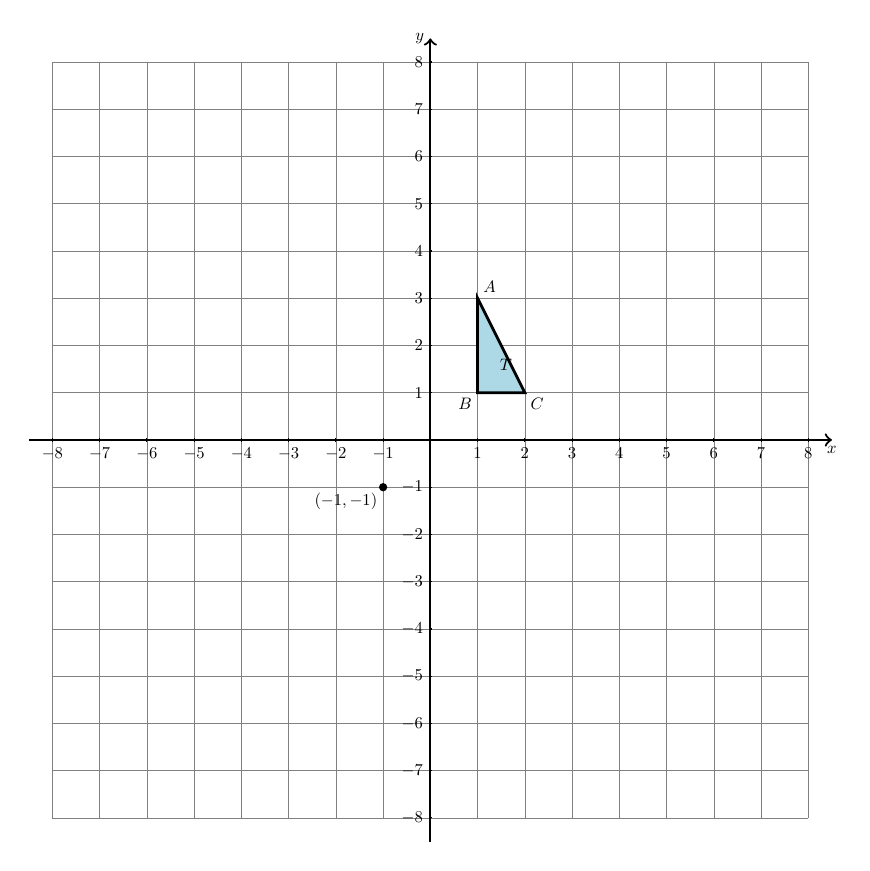
\begin{tikzpicture}[scale=0.6, transform shape]
    \definecolor{borderColour}{HTML}{000000}
    \definecolor{fillColourT}{HTML}{ADD8E6}

    \def\axisLimit{8}

    % Draw grid
    \draw[step=1cm,gray,very thin] (-\axisLimit,-\axisLimit) grid (\axisLimit,\axisLimit);

    % Draw axes
    \draw[thick,->] (-\axisLimit-0.5,0) -- (\axisLimit+0.5,0) node[anchor=north] {$x$};
    \draw[thick,->] (0,-\axisLimit-0.5) -- (0,\axisLimit+0.5) node[anchor=east] {$y$};

    % Label x-axis and y-axis
    \foreach \x in {-\axisLimit,...,-1,1,2,...,\axisLimit}
        \draw (\x cm,1pt) -- (\x cm,-1pt) node[anchor=north] {$\x$};
    \foreach \y in {-\axisLimit,...,-1,1,2,...,\axisLimit}
        \draw (1pt,\y cm) -- (-1pt,\y cm) node[anchor=east] {$\y$};

    % Define vertices of T
    \coordinate (A) at (1,3);
    \coordinate (B) at (1,1);
    \coordinate (C) at (2,1);

    % Draw T
    \filldraw[fill=fillColourT, draw=borderColour, line width=1pt] (A) -- (B) -- (C) -- cycle;
    \node[above right] at (A) {$A$};
    \node[below left] at (B) {$B$};
    \node[below right] at (C) {$C$};
    \node at (1.6,1.6) {$T$};

    % Mark centre of enlargement
    \fill[black] (-1,-1) circle (2.5pt);
    \node[below left] at (-1,-1) {$(-1,-1)$};

\end{tikzpicture}
\end{center}

\noindent On a copy of this diagram, draw and label triangle $T'$, the image of $T$ after this enlargement, and state the coordinates of its vertices $A'$, $B'$ and $C'$.

\vspace{5cm}

\begin{flushright}
    \answerplain{4}
\end{flushright}
\end{question}
